\subsubsection*{Casos de Prueba}
\addcontentsline{toc}{subsubsection}{Casos de Prueba}

Generamos casos de pruebas en base al primer análisis de los escenarios típicos de las entradas. Para esto realizamos pruebas con entradas de 200 edificios cada una con las siguientes configuraciones:

\begin{enumerate}[(a)]
	\item Edificios todos separados.
	\item Edificios uno a continuacion del otro (compartiendo bordes, el finalizar uno comenzaba el otro imediatamente).
	\item Edificios cruzados en forma de escalera ascendete.
	\item Edificios cruzados en forma de escalera descendente.
	\item Edificios cruzados en forma de piramide.
	\item Un edificio que queda por encima de todos los otros.
	\item Una entrada aleatoria.
\end{enumerate}

$
\begin{array}{cc}
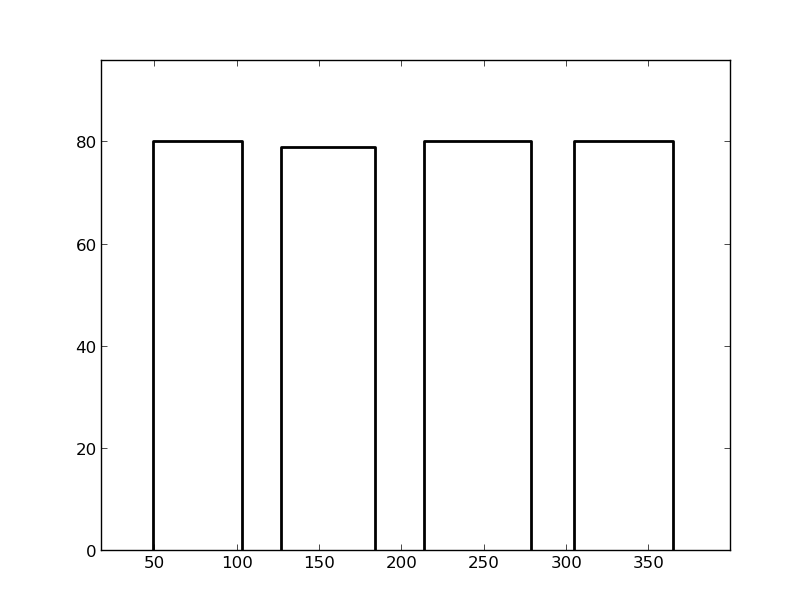
\includegraphics[scale=0.35]{./imagenes/ej2_edificiosSeparados.png}&
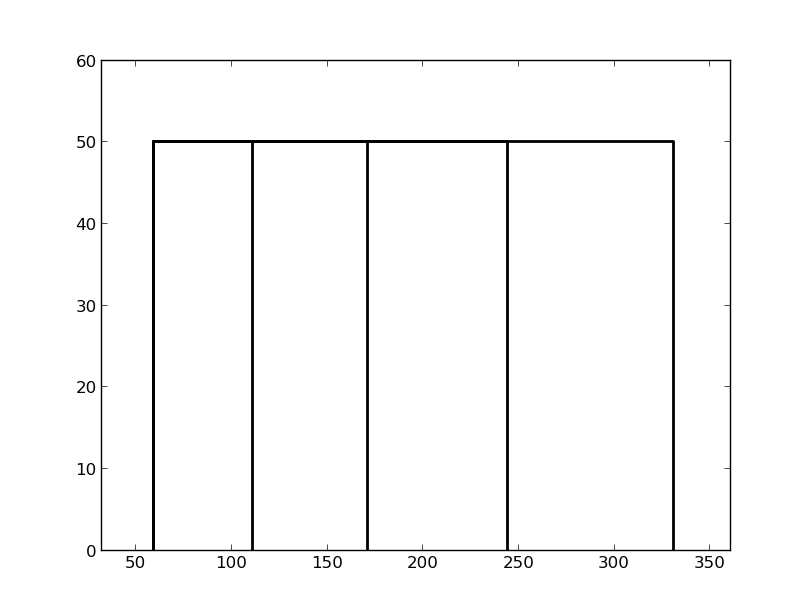
\includegraphics[scale=0.35]{./imagenes/ej2_edificiosJuntos.png}&
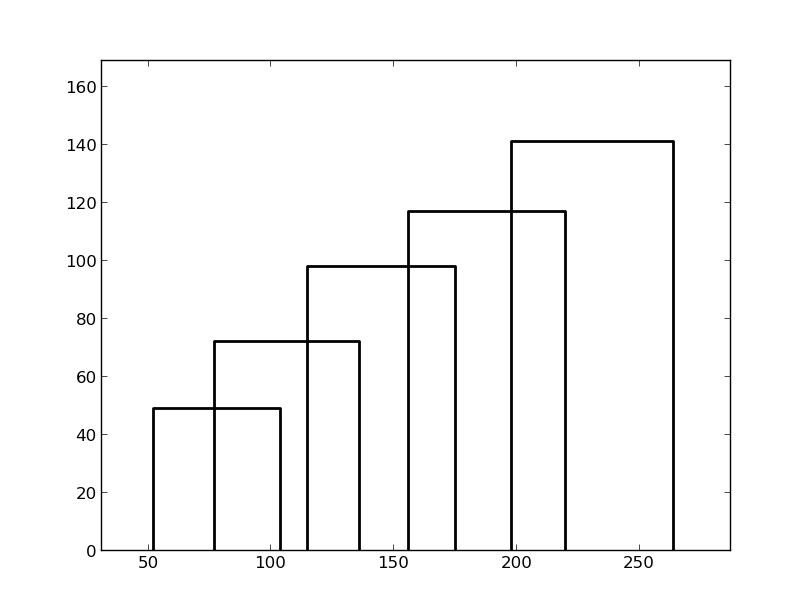
\includegraphics[scale=0.35]{./imagenes/ej2_edificiosSubiendo.png}&
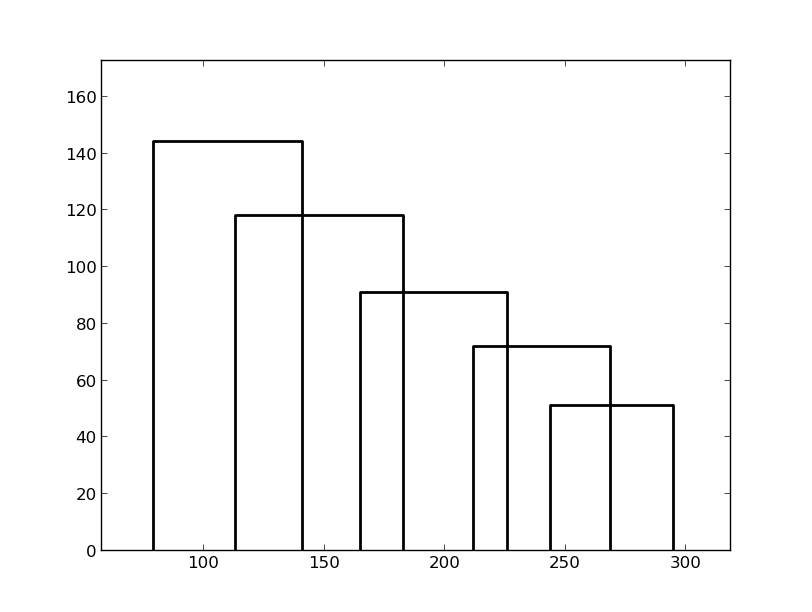
\includegraphics[scale=0.35]{./imagenes/ej2_edificiosBajando.png}
\end{array}
$

$
\begin{array}{cc}
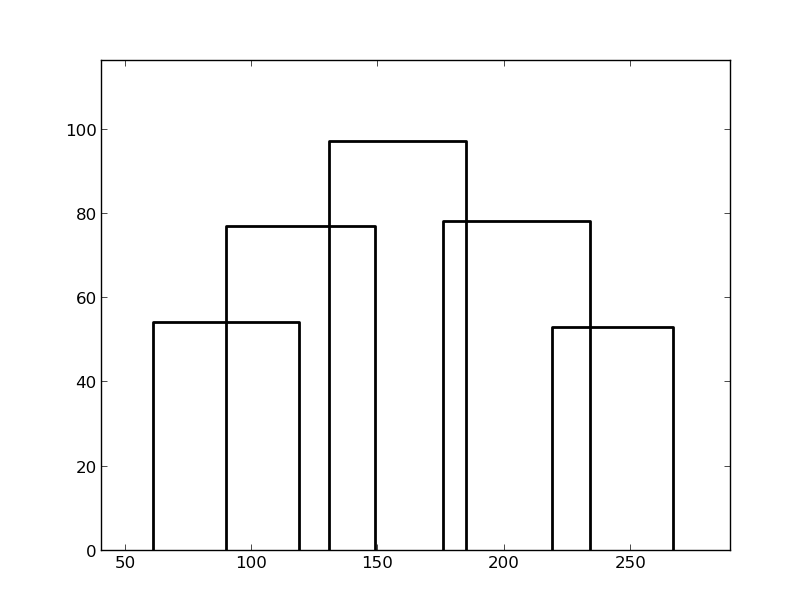
\includegraphics[scale=0.35]{./imagenes/ej2_edificiosPiramide.png}&
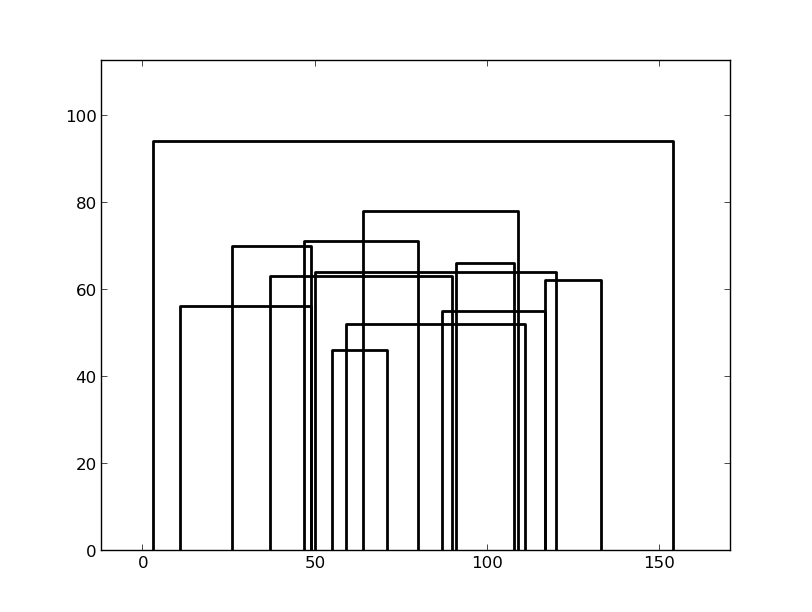
\includegraphics[scale=0.35]{./imagenes/ej2_edificiosOpacando.png}&
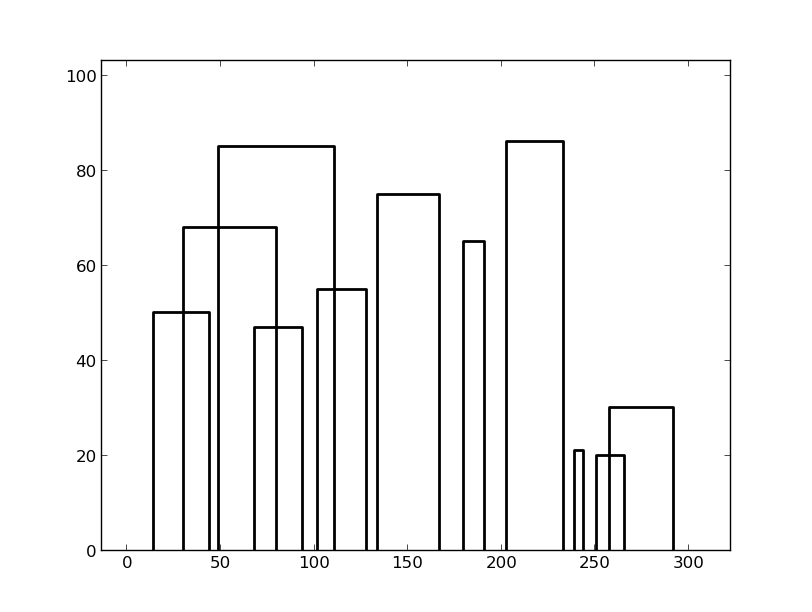
\includegraphics[scale=0.35]{./imagenes/ej2_edificiosAleatorios.png}
\end{array}
$

Luego de estos experimentos, pudimos evidenciar que la disposición y cararcteristicas de los edificios no influye en el rendimiento del algoritmo como era de esperarse.


\subsubsection*{Performance}
\addcontentsline{toc}{subsubsection}{Performance}

Para realizar el análisis de performance generamos instancias de test pseudoaleatorias determinadas con la semilla que recibe como parámetro el ejecutable test.

Esto genera 200 instancias de edificios pseudoaleatorios acotados en altura y longitud, siempre con comienzo $<$ fin del edificio.

\begin{figure}[H]
\begin{center}
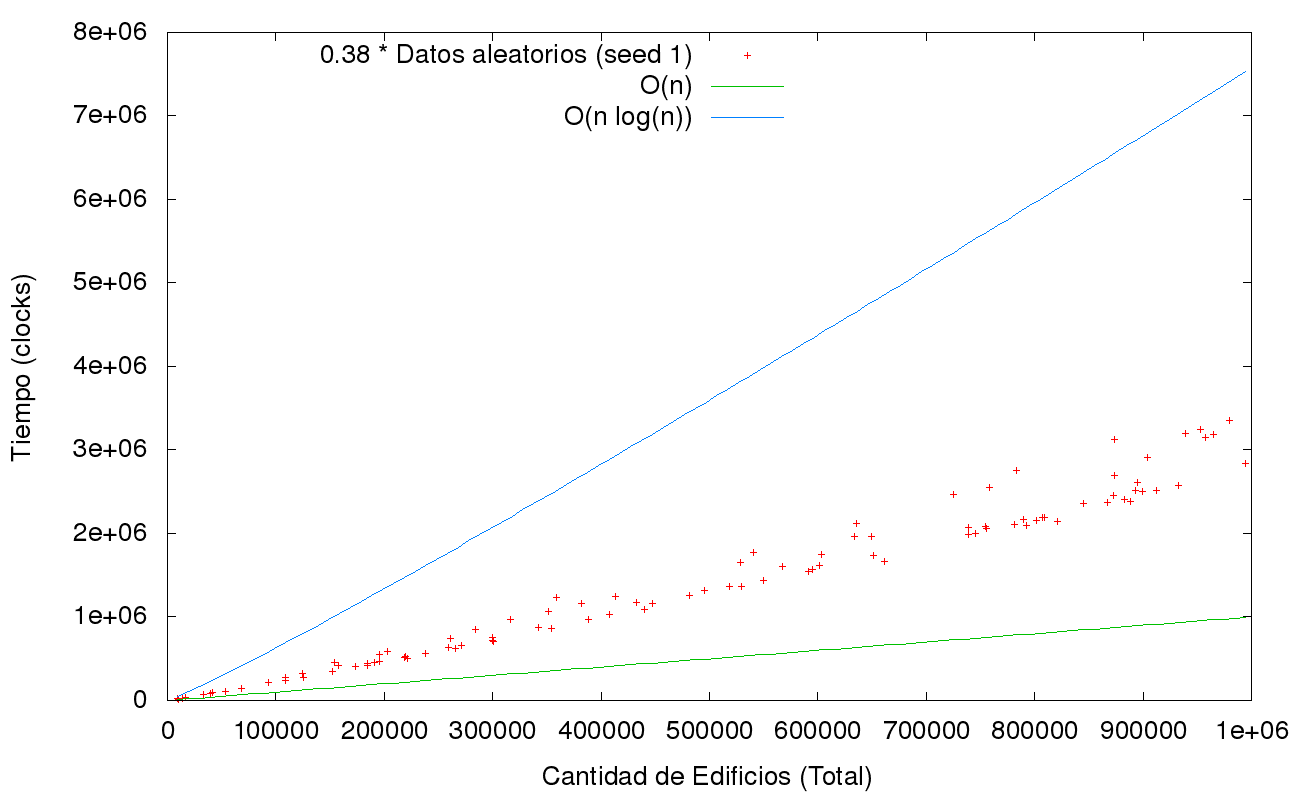
\includegraphics[scale=0.35]{./imagenes/ej2_chartRendimiento.png}
\caption{Gr\'afico de tiempo en funci\'on de la cantidad de edificios.}
\end{center}
\end{figure}

Para evidenciar que la complejidad es la que propusimos en el análisis teórico en el gráfico agregamos dos funciones para acotar superior e inferiormente. Una O(nlog(n)) y la otra O(n).
Y también dividimos a nuestros resultados por n log(n) para poder verla como una recta.